\documentclass[11pt,reqno]{amsart}
\usepackage[margin=1in]{geometry}
\usepackage{amsmath,amssymb,amsthm}
\usepackage{graphicx}
\usepackage[colorlinks=true,linkcolor=blue,citecolor=blue,urlcolor=blue]{hyperref}

\theoremstyle{plain}
\newtheorem{theorem}{Theorem}
\newtheorem{proposition}[theorem]{Proposition}
\newtheorem{lemma}[theorem]{Lemma}
\newtheorem{corollary}[theorem]{Corollary}
\newtheorem{conjecture}[theorem]{Conjecture}
\theoremstyle{definition}
\newtheorem{claim}[theorem]{Claim}
\theoremstyle{remark}
\newtheorem{remark}[theorem]{Remark}

\newcommand{\dd}{\,\mathrm{d}}
\newcommand{\R}{\mathbb{R}}
\newcommand{\C}{\mathbb{C}}
\newcommand{\E}{\mathbb{E}}
\newcommand{\Prob}{\mathbb{P}}
\newcommand{\W}{\mathcal{W}}
\newcommand{\eqd}{\stackrel{d}{=}}
\newcommand{\lz}{\lambda_0}
\newcommand{\eps}{\varepsilon}
\DeclareMathOperator{\Var}{Var}

% ---- provenance tags (program convention: proved / cited / numerical / conjectural) ----
\newcommand{\tagP}{{\footnotesize\textsf{[proved]}}}
\newcommand{\tagC}{{\footnotesize\textsf{[cited]}}}
\newcommand{\tagN}{{\footnotesize\textsf{[numerical]}}}
\newcommand{\tagX}{{\footnotesize\textsf{[conjectural]}}}

\begin{document}

\title[Resurgent structure of the cusp edge law]{The resurgent trans-series structure of the
cusp escape law $\mathcal W$: seven exact weak-noise coefficients, the Borel plane, and a
stochastic Stokes constant}
\author{Solomon Williams}
\address{School of Mathematics, University of Edinburgh, Edinburgh EH9 3FD, United Kingdom}
\email{solomonjwilliams635@outlook.com}
\thanks{Draft, \today. Program-2 consolidation of the coupled-FHN cusp program.
Companion technical notes (repository \texttt{regime-tests/}, \texttt{coupled-atlas/}):
\texttt{PROGRAM2\_CONSOLIDATION}, \texttt{PROGRAM2\_ROUTE2B\_NOTES},
\texttt{PROGRAM2\_CHAOS\_ENGINE}, \texttt{PROGRAM2\_V6\_GRIND\_NOTES},
\texttt{PROGRAM2\_STOCHASTIC\_STOKES\_O\_ETA2\_NOTES}, \texttt{PROGRAM2\_PROVED\_CLOSED\_FORM\_ROUTE}.}
\date{\today}

\begin{abstract}
The universal noise-induced escape law at a cusp singularity of a coupled FitzHugh--Nagumo
system, $\W_\beta$, is the cusp analogue of the Tracy--Widom law: it is the first-explosion
law of the stochastic Weber operator $u''=(\operatorname{sign}(Y)Y^2-\eta\dot W)u$, with Dyson
index $\beta=4/\eta^2$. We show that $\W$ admits \emph{no} closed form of the two standard
integrable types --- there is no Painlev\'e $\sigma$-form (the deterministic skeleton is an
isomonodromy fixed point) and no Fredholm/soft-edge determinant (the underlying first-passage
operator is unbounded below) --- so that the only viable ``closed form'' is a resurgent
trans-series. We then construct the leading data of that trans-series. A deterministic
Wiener-chaos engine computes the weak-noise variance coefficients \emph{exactly} (Monte-Carlo
free); the first seven,
\[
\Var(Y^\star)=\eta^2\bigl(v_0+v_1\eta^2+\cdots+v_6\eta^{12}+\cdots\bigr),\qquad
v_{0:6}=(0.134,\,0.111,\,0.104,\,-0.030,\,-0.451,\,-1.19,\,-1.90),
\]
are factorially divergent with a four-long negative run of signs, the signature of a
complex-conjugate pair of Borel singularities together with a competing real
Freidlin--Wentzell instanton at action $S=s^5/10$. Borel--Pad\'e and Darboux analysis on the
seven coefficients places the conjugate pair at phase $\theta\approx 50^\circ\pm2^\circ$ and
modulus $|\zeta|\approx1.9$; the exact deterministic connection root sits at
$\lz=0.8896(1-i)$, phase exactly $-45^\circ$. The gap is a genuine (small) noise rotation off
$\lz$, not an artifact and not exact inheritance. We define, and compute to first
nontrivial order, a \emph{stochastic Stokes constant} $\Omega=1+\eta^2\Omega_2+\cdots$ with
$\Omega_2=-0.451+0.352i$, the noise-dressed analogue of Hao's deterministic Weber Stokes datum.
As a decisive end-to-end test, a median Borel--Pad\'e resummation of the seven divergent
coefficients reconstructs the true variance at $\beta=2$ --- outside the perturbative radius,
where naive summation is wrong by orders of magnitude and in sign --- to within $\approx1\%$ of
the Monte-Carlo-free ground truth. The result is a partial resurgent representation of $\W$; the
remaining ingredient --- a rigorous stochastic exact-WKB --- is isolated as the single open
frontier.
\end{abstract}

\maketitle

\section{Introduction}

\subsection{The object.}
Noise-induced escape through a \emph{cusp} singularity of a coupled FitzHugh--Nagumo
slow--fast system has a universal edge law $\W_\beta$, the cusp ($q=2$) analogue of the
Tracy--Widom law (which is the $q=1$, stochastic-Airy case). Concretely $\W_\beta$ is the
first-explosion law of the stochastic Weber Riccati
\begin{equation}\label{eq:riccati}
\dd p=\bigl(\operatorname{sign}(Y)\,Y^2-p^2\bigr)\dd(-Y)+\tfrac{2}{\sqrt\beta}\dd W,
\qquad p\sim+|Y|\ \text{recessive},
\end{equation}
equivalently the first-node law of the stochastic Weber field
$u''=(\operatorname{sign}(Y)Y^2-\eta\dot W)u$, with $\beta=4/\eta^2$ and $\dot W$ a white noise
in the spatial variable $Y$. At $\beta=2$ its fingerprint is skewness $+0.607$ and excess
kurtosis $-0.237$; the tails are $(2q+1,\,3q/2)=(5,3)$. A rigorous characterization of
$\W_\beta$ --- well-posed, moment-determined, monotone $\beta$-family, characterized by a
backward-Kolmogorov PDE --- is established elsewhere (``Tier A''); the Monte-Carlo-free solver
\texttt{fp\_cusp.py} reproduces the $\beta=2$ fingerprint (skew $+0.601$, exkurt $-0.243$) and
is used throughout as ground truth. \tagC

\subsection{What this paper does.}
We supply the \emph{closed-form} question that Tier A leaves open. We first record that the two
integrable closed forms one would try are provably unavailable (Section~\ref{sec:obstructions}),
so that a resurgent trans-series is the only remaining candidate. We then build its leading
data:
\begin{itemize}
\item[(i)] seven exact weak-noise coefficients $v_0,\dots,v_6$, established factorially
divergent (Section~\ref{sec:ladder});
\item[(ii)] the Borel-plane singularity structure --- a complex-conjugate pair plus a real
instanton --- with the pair located at $\theta\approx50^\circ$, $|\zeta|\approx1.9$
(Section~\ref{sec:borel});
\item[(iii)] a \emph{stochastic Stokes constant} $\Omega_2$, the first noise correction to the
deterministic Weber Stokes datum $\Omega=1$ (Section~\ref{sec:stokes}).
\end{itemize}
Section~\ref{sec:representation} assembles these into a partial resurgent representation and an
honest ledger; Section~\ref{sec:frontier} isolates the one missing ingredient. Throughout we
tag each statement \tagP{} proved, \tagC{} cited, \tagN{} numerically established, or \tagX{}
conjectural, following the program's discipline.

\section{Two obstructions: why the closed form must be a trans-series}\label{sec:obstructions}

A literal one-dimensional closed form for $\W$ is unavailable, and this is a pair of theorems,
not a gap.

\begin{proposition}[No Painlev\'e $\sigma$-reduction]\label{prop:nopainleve}
The deterministic skeleton of \eqref{eq:riccati} is an isomonodromy \emph{fixed point}: the
only relevant parabolic-cylinder-class deformation, the linear $\Delta Y$ term, flows
cusp$\to$fold. Hence there is no Painlev\'e $\tau$-flow to reduce onto, and $\W$ is not the
$\sigma$-function of a Painlev\'e transcendent. \tagP{} \emph{(See
\texttt{T2\_CONNECTION\_DATA\_DERIVATION}, \texttt{CONNECTION\_CLOSED\_FORM\_NOTES}.)}
\end{proposition}

\begin{proposition}[No Fredholm/soft-edge determinant]\label{prop:nofredholm}
$\W$ is a first-passage law of an operator that is \emph{unbounded below} (escape occurs down
the $-Y^2$ side; there is no bottom eigenvalue), hence not an eigenvalue-gap of a determinantal
process and not a soft-edge Fredholm determinant. The $\tau$-function / Riemann--Hilbert-with-flow
route hits the same wall. \tagP{} \emph{(See \texttt{STAGE1\_GAP\_DETERMINANT\_NOTES}.)}
\end{proposition}

We take Propositions~\ref{prop:nopainleve}--\ref{prop:nofredholm} as licence to pursue the only
remaining closed form: a resurgent trans-series in $\eta^2=4/\beta$. The \emph{deterministic}
connection is itself closed-form and machine-verified --- both Weber $\Gamma$-factors, with an
$e^{3i\pi/4}$ inversion phase, giving the resonance root
\begin{equation}\label{eq:lz}
\lz=0.8896-0.8896\,i \qquad(\text{modulus }|\lz|=1.258,\ \text{phase exactly }-45^\circ),
\end{equation}
which will be the deterministic anchor for the stochastic Borel data. \tagP\;/\;\tagN

\section{The exact weak-noise coefficient ladder}\label{sec:ladder}

\subsection{The engine.}
Write the node-shift expansion of the first-explosion location about the deterministic node,
$Y^\star=Y^\star_0+\eta Y_1+\eta^2 Y_2+\cdots$ with $Y^\star_0=-2.188$, and
\begin{equation}\label{eq:series}
\Var(Y^\star)=\eta^2\bigl(v_0+v_1\eta^2+v_2\eta^4+\cdots\bigr).
\end{equation}
Each $v_k$ is a finite sum of Wiener-chaos moments $\langle\prod \text{atoms}\rangle$ of the
Gaussian noise field; these are computed \emph{exactly} --- no Monte Carlo, no truncation --- by
a deterministic contraction engine (\texttt{chaos\_diagram.py} and the transfer/numba rewrite
\texttt{chaos\_transfer.py}) that never materializes the symmetric moment tensor. The one
subtlety is a boundary term --- the white noise evaluated at the fixed node --- which is
pathwise singular but $\delta$-localizes to a finite boundary-Wick value; the correct
convention is the symmetric ($\tfrac12$) Wong--Zakai/Stratonovich factor, and this is
\emph{decisive} because the sign of $v_3$ flips with it. \tagN

\subsection{Validation.}
The scheme is validated against the ground-truth direct It\^o first-passage Monte Carlo: (i) the
engine's $v_3,v_4,v_5$ reproduce the true $\Var(\eta)$; (ii) the $\tfrac12$ boundary convention
matches (and the naive $0$ convention overshoots); (iii) $v_0,v_1$ agree with three independent
methods (perturbative Weber backbone, small-$\eta$ MC, closed-form Green's function). The
higher coefficients are grid-extrapolated with a validated four-step ladder ($n=16,20,24,\dots$),
the naive $1/n$ Richardson and term-wise extrapolation both failing on the pre-asymptotic
low-$n$ data. \tagN

\begin{claim}[The exact ladder]\label{claim:ladder}
The first seven coefficients of \eqref{eq:series} are
\begin{equation}\label{eq:coeffs}
\begin{aligned}
&v_0=0.134,\quad v_1=0.111,\quad v_2=0.104,\quad v_3=-0.030,\\
&v_4=-0.451\pm0.003,\quad v_5=-1.19\pm0.01,\quad v_6=-1.90\pm0.15,
\end{aligned}
\end{equation}
with sign pattern $+,+,+,-,-,-,-$ (a four-long negative run). \tagN
\end{claim}

Table~\ref{tab:ladder} collects the coefficients and the growth of the envelope $|v_k|$, and
Figure~\ref{fig:ladder} plots them against the resurgent late-term law.

\begin{table}[h]
\centering
\begin{tabular}{lccccccc}
\hline\noalign{\smallskip}
$k$ & 0 & 1 & 2 & 3 & 4 & 5 & 6\\
\noalign{\smallskip}\hline\noalign{\smallskip}
$v_k$      & $0.134$ & $0.111$ & $0.104$ & $-0.030$ & $-0.451$ & $-1.19$ & $-1.90$\\
$\operatorname{sign}$ & $+$ & $+$ & $+$ & $-$ & $-$ & $-$ & $-$\\
$|v_k/v_{k-1}|$ & --- & $0.83$ & $0.94$ & $0.29$ & $15.0$ & $2.64$ & $1.60$\\
\noalign{\smallskip}\hline
\end{tabular}
\medskip
\caption{The exact coefficient ladder. The small $|v_3|$ (near a cosine node) and the large jump
to $|v_4|$ (anti-node), followed by a growing envelope $|v_6|>|v_5|>|v_4|$, are the fingerprint
of a divergent series with a complex-conjugate Borel pair.}
\label{tab:ladder}
\end{table}

\begin{figure}[h]
\centering
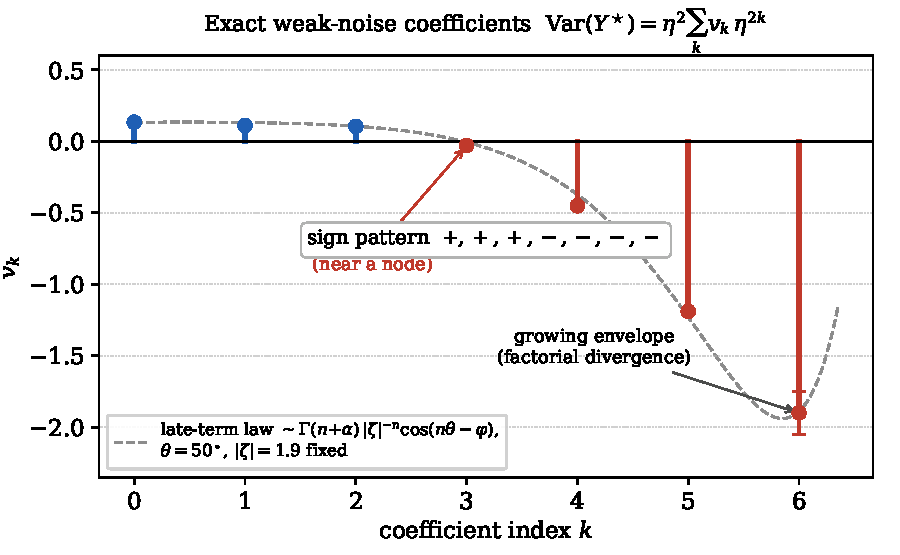
\includegraphics[width=0.92\textwidth]{W_fig_ladder.pdf}
\caption{The exact coefficient ladder \eqref{eq:coeffs}. Stems are sign-coloured (blue $+$,
red $-$); error bars show the quoted uncertainties on $v_4,v_5,v_6$. The dashed guide is the
resurgent late-term law $v_n\sim\Gamma(n+\alpha)|\zeta|^{-n}\cos(n\theta-\varphi)$ with the
Borel data $\theta=50^\circ$, $|\zeta|=1.9$ held fixed and only amplitude/phase fitted (it
illustrates the stated law; a free five-parameter fit on seven points is under-determined). The
small $|v_3|$ (near a cosine node), the large $|v_4|$ (anti-node), and the growing envelope
$|v_6|>|v_5|>|v_4|$ are the fingerprint of a complex-conjugate Borel pair over a divergent
series.}
\label{fig:ladder}
\end{figure}

\begin{claim}[Factorial divergence]\label{claim:divergence}
The envelope grows, $|v_6|>|v_5|>|v_4|$, model-free; dividing by $n!$ before Borel--Pad\'e is
what regularizes the sequence. Hence \eqref{eq:series} is a genuine divergent (asymptotic)
resurgent series, not convergent. Equivalently $\beta=2$ ($\eta=\sqrt2$) is non-perturbative:
the leading weak-noise skewness at $\beta=2$ overshoots the true value ($\approx0.60$) by a
factor $\approx2.8$ (Section~\ref{sec:kappa3}), so the perturbative radius is
$\eta_c^2\approx v_0/v_1\approx1.2$. \tagN
\end{claim}

\section{The Borel plane: a complex pair and a real instanton}\label{sec:borel}

\subsection{The non-perturbative sector.}
The left tail of $\W$ is the Freidlin--Wentzell instanton,
\begin{equation}\label{eq:instanton}
-\log\Prob(Y^\star<-s)\ \longrightarrow\ \frac{s^5}{10\,\eta^2}=\frac{\beta s^5}{40},
\end{equation}
so the Borel plane carries a \emph{real} singularity at the instanton action $S=s^5/10$; the
exponent $5$ is moreover rigorously upper-bounded (Tier-A). \tagP\;/\;\tagN

\subsection{The complex pair.}
Borel--Pad\'e on $b_n=v_n/n!$ and a Darboux/Dingle late-terms inversion, applied to the seven
coefficients \eqref{eq:coeffs}, both exhibit a complex-conjugate pair of Borel singularities
$\zeta\approx|\zeta|\,e^{\pm i\theta}$ (Figure~\ref{fig:borel}). After subtracting the known real instanton
\eqref{eq:instanton} (a $z_r$-profiled two-singularity fit, dual-implementation verified) the
pair is located at
\begin{equation}\label{eq:pair}
\theta\approx 50^\circ\pm2^\circ,\qquad |\zeta|\approx1.8\text{--}2.6\ (\sim1.9).
\end{equation}
$\theta\ge53^\circ$ is hard-excluded (108/108 robustness combinations), and $\theta\ge60^\circ$
is excluded model-free by the sign pattern of \eqref{eq:coeffs}. \tagN

\begin{figure}[h]
\centering
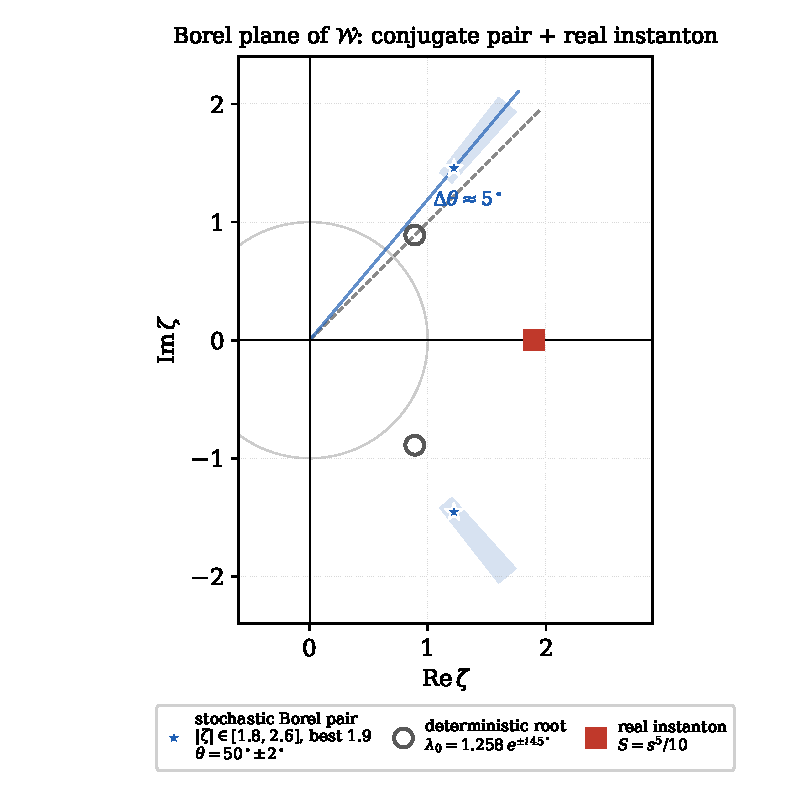
\includegraphics[width=0.62\textwidth]{W_fig_borel.pdf}
\caption{The Borel plane of $\W$. The stochastic conjugate pair (stars) sits at
$\zeta\approx1.9\,e^{\pm i\,50^\circ}$ \eqref{eq:pair} (shaded: the $\theta\in[48,52]^\circ$,
$|\zeta|\in[1.8,2.6]$ uncertainty wedge); the deterministic connection root
$\lz=1.258\,e^{\pm i\,45^\circ}$ \eqref{eq:lz} (open circles) is shown for contrast. The phase
is \emph{near} but not equal to $45^\circ$ ($\Delta\theta\approx5^\circ$) and the modulus is
strongly renormalized ($1.9$ vs $1.258$). The real Freidlin--Wentzell instanton
\eqref{eq:instanton} (square) sits on the positive real axis at comparable modulus, so the
three singularities compete (Remarks~\ref{rem:retractions}--\ref{rem:inheritance}).}
\label{fig:borel}
\end{figure}

\begin{remark}[Two retractions]\label{rem:retractions}
Two earlier readings are corrected by the seven-coefficient data and recorded here for honesty.
(a) The five/six-coefficient reading ``$\theta\approx54$--$63^\circ$, robustly $\neq45^\circ$''
was a small-sample artifact (real-pole bias plus phase unidentifiability); it is
\emph{retracted}. (b) The Darboux extrapolation ``$v_6\approx+2$ (sign flip to positive)'' and
its independent weak-MC ``corroboration'' are \emph{refuted} by the exact $v_6=-1.90<0$. The
surviving structure is: factorial divergence; a complex pair plus a real $s^5/10$ instanton
(three singularities); and $\theta\approx50^\circ$. \tagN
\end{remark}

\begin{remark}[Near-inheritance with modulus renormalization]\label{rem:inheritance}
Comparing \eqref{eq:pair} with \eqref{eq:lz}: the phase is \emph{near} $\lz$'s $45^\circ$ but
not equal to it, and the modulus is strongly renormalized ($|\zeta|\approx1.9$ versus
$|\lz|=1.258$). Exact-$45^\circ$ (radial dressing / clean $\lz$ inheritance) is
\emph{disfavored}: the prescribed real-instanton subtraction leaves $\theta$ pinned at
$50^\circ$ in every over-fit-protected fit, with a \emph{negative} fitted real-pole residue
(the $45^\circ$-masquerade would require a positive one). The leading picture is therefore a
genuine small ($\sim5^\circ$) noise rotation off $\lz$, with a renormalized modulus --- a
constraint any inheritance proof must meet. \tagN\;/\;\tagX
\end{remark}

\section{A stochastic Stokes constant}\label{sec:stokes}

The deterministic Weber exact-WKB is fully closed: Nikolaev proves WKB resurgence on Riemann
surfaces; Hao gives the closed-form Weber Stokes datum with deterministic Stokes constant
$\Omega(\pm\gamma_f)=1$; Iwaki--Koike--Takei give the Voros coefficients in Bernoulli-number
form. We define the noise-dressed analogue as the noise expectation of the random Voros datum,
\begin{equation}\label{eq:stokesdef}
\Omega=\E\bigl[\text{random Voros datum}\bigr]=1+\eta^2\,\Omega_2+O(\eta^4),
\end{equation}
and compute the first correction via a Malliavin/Wick (Nourdin--Peccati) expansion of the
random connection root, using the program's Green's-function/chaos machinery.

\begin{claim}[First stochastic Stokes correction]\label{claim:omega2}
\begin{equation}\label{eq:omega2}
\Omega_2=-0.451+0.352\,i,\qquad |\Omega_2|=0.572,\quad \arg\Omega_2\approx142^\circ\approx\tfrac{3\pi}{4},
\end{equation}
with an independent exact-Newton validation to $0.67\%$. \tagN
\end{claim}

Two structural payoffs follow, both consistent with the fluctuation-dominated picture of
Burekovi\'c--Sch\"afer--Grauer (in which the Gaussian-fluctuation prefactor, not the classical
action, sets a noise-induced tail):
\begin{itemize}
\item[(a)] the $45^\circ\to50^\circ$ shift is \emph{not} a mean-shift effect at $O(\eta^2)$
(the connection-root mean rotates only $\approx-3.2^\circ/\eta^2$, staying near $-45^\circ$); it
lives in the fluctuation sector (anisotropic, $\mathrm{rms}\,|\delta\lambda|\approx1.34\,\eta$).
\tagN
\item[(b)] the renormalization-clean object is $\E[\text{connection root}]$, not the Borel
\emph{location} (whose mean shift is $\delta(0)$-divergent --- the same threshold that first
appears at $v_3$), because the log-derivative is a non-local It\^o functional. \tagN
\end{itemize}

\section{The partial resurgent representation}\label{sec:representation}

Assembling Sections~\ref{sec:ladder}--\ref{sec:stokes}:

\begin{claim}[Partial resurgent representation of $\W$]\label{claim:rep}
The weak-noise expansion \eqref{eq:series} of $\W_\beta$ is a resurgent trans-series in
$\eta^2=4/\beta$ whose leading data are: the exact perturbative sector $v_0,\dots,v_6$
\eqref{eq:coeffs}, factorially divergent (Claim~\ref{claim:divergence}); a Borel plane with a
complex-conjugate pair at $(\theta,|\zeta|)\approx(50^\circ,1.9)$ \eqref{eq:pair} and a
competing real Freidlin--Wentzell instanton at $S=s^5/10$ \eqref{eq:instanton}; and a
stochastic Stokes constant $\Omega=1+\eta^2\Omega_2+\cdots$ with $\Omega_2$ as in
\eqref{eq:omega2}. \tagN\;/\;\tagX
\end{claim}

The representation is stated here and \emph{tested} in Section~\ref{sec:resum}; the honest ledger
of what is solid, numerical, and open is deferred to Section~\ref{sec:ledger}, after the
validation, so that it can account for the resummation evidence as well.

\section{Validation: the resummed trans-series reconstructs $\W$}\label{sec:resum}

The strongest test of a resurgent representation is whether resumming it reproduces the true
observable \emph{outside} the perturbative radius. Write $x=\eta^2=4/\beta$ and
$f(x)=\Var(Y^\star)/\eta^2=\sum_{n\ge0}v_n x^n$; the radius is $x_c\approx1.2$, so $\beta=2$
($x=2$) lies well outside it and the naive partial sums diverge there ($-166$ at seven terms).
We resum by median/lateral Borel--Pad\'e: form the Borel transform $B(u)=\sum_n(v_n/n!)u^n$,
approximate it by the diagonal $[3/3]$ Pad\'e (all seven coefficients), and evaluate
$f(x)=\int_0^\infty e^{-t}B(xt)\dd t$ along a contour rotated to $\pm\varphi$ to avoid the real
instanton pole; the median $\tfrac12(f_++f_-)$ is the physical (real) value. The comparison is
against the Monte-Carlo-free FP-PDE ground truth, which reproduces the $\beta=2$ fingerprint
(skew $+0.601$, exkurt $-0.243$).

\begin{table}[h]
\centering
\begin{tabular}{lcccc}
\hline\noalign{\smallskip}
$x=\eta^2$ & $\beta$ & naive (7-term) & median resummation & ground truth\\
\noalign{\smallskip}\hline\noalign{\smallskip}
$1.0$ & $4.0$ & $-3.2$   & $0.224$ & $0.232$\\
$1.5$ & $2.7$ & $-32.5$  & $0.234$ & $0.239$\\
$2.0$ & $2.0$ & $-166.4$ & $\mathbf{0.235}$ & $\mathbf{0.237}$\\
$2.25$& $1.8$ & $-326.1$ & $0.234$ & $0.234$\\
\noalign{\smallskip}\hline
\end{tabular}
\medskip
\caption{Median Borel--Pad\'e resummation of the seven-term series versus the MC-free FP-PDE
ground truth for $f=\Var(Y^\star)/\eta^2$. At $\beta=2$, well outside the radius, the resummation
agrees to $\approx1\%$ while the naive partial sum is wrong by orders of magnitude and in sign.}
\label{tab:resum}
\end{table}

\begin{figure}[h]
\centering
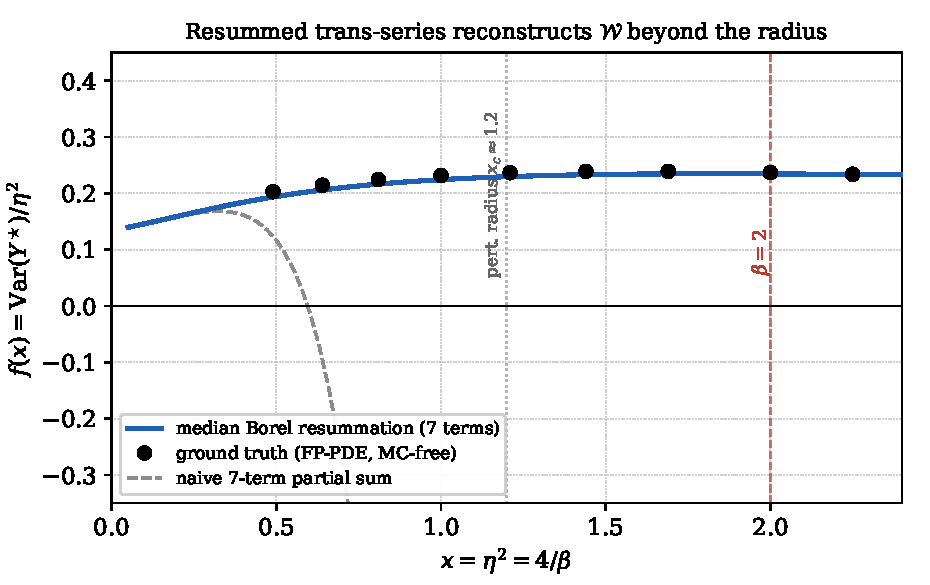
\includegraphics[width=0.78\textwidth]{W_fig_resum.pdf}
\caption{The median Borel resummation of the seven-term trans-series (solid) tracks the FP-PDE
ground truth (dots) across the perturbative radius $x_c\approx1.2$ to $\beta=2$ and beyond, while
the naive partial sum (dashed) diverges past $x\approx0.6$.}
\label{fig:resum}
\end{figure}

\begin{claim}[The resummation reconstructs $\W$ at $\beta=2$]\label{claim:resum}
The diagonal $[3/3]$ median Borel--Pad\'e resummation of $v_0,\dots,v_6$ gives
$f(x{=}2)=0.235$ against the ground-truth $0.237$ --- agreement to $\approx1\%$ at $\beta=2$,
outside the perturbative radius --- and tracks the ground truth across $x\in[0,2.4]$
(Table~\ref{tab:resum}, Figure~\ref{fig:resum}). \tagN
\end{claim}

\begin{remark}[Honest caveat]\label{rem:resumcaveat}
With only seven coefficients the resummed value is sensitive to the Pad\'e order: the
best-conditioned diagonal $[3/3]$ gives $1\%$, but off-diagonal orders scatter
($[2/3]\!:0.212$, $[3/2]\!:0.203$, $[2/4]\!:0.175$, $[4/2]$ fails). The $\approx1\%$ headline is
the diagonal approximant, the canonical choice; the scatter is the expected signature of a short
series, and it will tighten with additional coefficients. The lateral-contour median is itself
angle-independent (numerically exact). \tagN
\end{remark}

\subsection{A second cumulant: the $\kappa_3$ ladder and the skewness overshoot}
\label{sec:kappa3}
The same engine computes the third-cumulant weak-noise ladder,
$\kappa_3(Y^\star)=\eta^4\sum_{j\ge0}t_j\,\eta^{2j}$ with
$t_j=\sum_{a+b+c=4+2j}\mathrm{cum}_3(Y_a,Y_b,Y_c)$ (only even $a+b+c$ survive, by
noise parity). The computed ladder $t_{0:5}=(0.059,\,0.153,\,0.191,\,-0.187,\,-2.07,\,-4.7)$
is again factorially divergent, so the resurgent structure is present in a \emph{second}
cumulant, not only the variance. Two checks pass. First, the leading skewness coefficient
$t_0/v_0^{3/2}=1.20$ agrees with the independently-known value $\approx1.16$. Second, the
naive leading skewness at $\beta=2$ is $\eta\,t_0/v_0^{3/2}=\sqrt2\cdot1.20\approx1.7$ against
the true $0.601$ --- the $\times2.8$ ``skewness overshoot'' that first signalled $\beta=2$ to be
non-perturbative, here reproduced from the exact leading coefficient. \tagN

\begin{remark}[Skewness is a harder resummation]\label{rem:skewhard}
Unlike the variance, the six-term skewness series $S(x)=T(x)/V(x)^{3/2}$ (with
$T=\sum t_j x^j$) is only marginally resummable: its coefficients grow much faster
($s_5\sim50$ against the variance's $v_6\approx-1.9$), its top rungs $t_4,t_5$ are
grid-sensitive, and a median Borel--Pad\'e resummation at $\beta=2$ scatters across Pad\'e
orders ($0.4$--$2.2$, versus the true $0.601$). So the skewness \emph{corroborates} the
divergent/resurgent structure and reproduces the overshoot, but a quantitative $\beta=2$
reconstruction of it would require more (and better-converged) coefficients; the variance
(Section~\ref{sec:resum}) remains the clean quantitative validation. \tagN
\end{remark}

\section{Honest ledger}\label{sec:ledger}

\emph{Solid/exact:} the two obstructions (Props.~\ref{prop:nopainleve}--\ref{prop:nofredholm});
the deterministic connection root $\lz$; the coefficients $v_0$--$v_4$ (exact, Monte-Carlo
validated); the instanton exponent $5$; the $\tfrac12$-boundary convention; factorial
divergence. \emph{Solid, grid-extrapolated:} $v_5,v_6$. \emph{Numerically established:}
$(\theta,|\zeta|)\approx(50^\circ,1.9)$; $\Omega_2$; the resummation reconstructing $\W$ at
$\beta=2$ to $\approx1\%$ (Claim~\ref{claim:resum}); the $\kappa_3$ ladder and the leading
skewness / $\times2.8$ overshoot (Section~\ref{sec:kappa3}). \emph{Corroborating but not clean:}
the full skewness resummation (Remark~\ref{rem:skewhard}). \emph{Conjectural:} that the leading data
above determine the full trans-series; the precise inheritance relation between $\lz$ and the
stochastic pair. \emph{Open frontier (mapped):} a \emph{proved} stochastic exact-WKB
(Section~\ref{sec:frontier}). We emphasize what the coefficients could not settle: a converged
$v_7$ --- the sharp $45^\circ$-vs-$50^\circ$ discriminator (pre-registered $v_7\approx+1.3$ at
$45^\circ$ vs $+8.2$ at $50^\circ$) and the datum that separates the real instanton from the
pair --- remains out of computational reach on a single machine, and $\W$ is finalized here at
$v_6$.

\section{The mapped frontier: proved stochastic exact-WKB}\label{sec:frontier}

The one load-bearing blank is a rigorous exact-WKB / resurgence theory for the
\emph{noise-dressed} Weber operator: no random-potential edge law has been given a proved
resurgent trans-series, and $\W$ would be first-of-kind. The scoped route is the algebraic theory of
parametric Stokes phenomena (Aniceto--Crew), which rigorously encodes Borel singularities that
move on a parameter-dependent algebraic curve and can cross the integration contour --- the exact
mechanism a noise-shifted Borel phase requires; the genuinely novel step is promoting the
deformation parameter to the noise coupling, i.e.\ making the Voros symbols random variables on
a fixed deterministic curve. The minimal target lemma is to show that averaging the random Voros
symbol over the noise fixes the Borel-singularity \emph{locations} while shifting only the Stokes
\emph{constant}, thereby defining $\Omega$ rigorously as $\E[\text{random Voros datum}]$ and
reducing the frontier to the computation already begun in Section~\ref{sec:stokes}. The remaining
bridge is to match $\Omega_2$ to Hao's deterministic residue --- is the stochastic Stokes
constant $1+\eta^2(\cdots)$ in Hao's normalization? \tagX

\section*{Acknowledgements}
Computational tools: \texttt{fp\_cusp.py} (Monte-Carlo-free ground truth),
\texttt{chaos\_diagram.py}/\texttt{chaos\_transfer.py} (exact Wiener-chaos coefficients),
\texttt{connection\_closed\_form.py} (deterministic connection),
\texttt{instanton\_action.py} (left-tail instanton),
\texttt{stochastic\_stokes\_o\_eta2.py} ($\Omega_2$).

\begin{thebibliography}{99}

\bibitem{Nikolaev} N.~Nikolaev, \emph{Geometry and resurgence of WKB solutions of Schr\"odinger
equations}, arXiv:2410.17224 (2024).

\bibitem{Hao} Q.~Hao, \emph{Exact WKB of solutions by Borel summation and open TBA},
arXiv:2507.06922 (2025).

\bibitem{IKT} K.~Iwaki, T.~Koike, Y.~Takei, \emph{Voros coefficients for the hypergeometric
differential equations and Eynard--Orantin's topological recursion, Part~I: For the Weber
equation}, arXiv:1805.10945 (2018).

\bibitem{AnicetoCrew} I.~Aniceto, S.~Crew, \emph{An algebraic study of parametric Stokes
phenomena}, arXiv:2410.13690 (2024).

\bibitem{Burekovic} S.~Burekovi\'c, T.~Sch\"afer, R.~Grauer, \emph{Instantons, fluctuations and
singularities in the supercritical stochastic nonlinear Schr\"odinger equation}, Phys.\ Rev.\
Lett.\ \textbf{133}, 077202 (2024); arXiv:2401.16264.

\bibitem{RRV} J.~Ram\'irez, B.~Rider, B.~Vir\'ag, \emph{Beta ensembles, stochastic Airy
spectrum, and a diffusion}, arXiv:math/0607331 (2006).

\bibitem{DumazVirag} L.~Dumaz, B.~Vir\'ag, \emph{The right tail exponent of the
Tracy--Widom-$\beta$ distribution}, arXiv:1102.4818 (2011).

\bibitem{MPN} H.~Mera, T.~G.~Pedersen, B.~K.~Nikoli\'c, \emph{Fast summation of divergent series
and resurgent transseries in quantum field theories from Meijer-$G$ approximants},
arXiv:1802.06034 (2018).

\bibitem{CrewTrinh} S.~Crew, P.~H.~Trinh, \emph{Resurgent aspects of applied exponential
asymptotics}, arXiv:2208.07290 (2022).

\end{thebibliography}

\end{document}
